% CHAOS OS: IEEE conference paper. Build: tectonic -X compile chaos-os-ieee.tex
% Figures: python docs/paper/make_figures.py ...; tables/macros: python docs/paper/make_tables.py
\documentclass[conference]{IEEEtran}
\IEEEoverridecommandlockouts
\usepackage[T1]{fontenc}
\usepackage{cite}
\usepackage{amsmath,amssymb}
\usepackage{graphicx}
\usepackage{booktabs}
\usepackage{multirow}
\usepackage{array}
\usepackage{xcolor}
\usepackage{url}
\usepackage[hidelinks]{hyperref}
\usepackage{balance}
\graphicspath{{figures/}}
\newcommand{\nTrials}{182}
\newcommand{\nAblation}{56}
\newcommand{\lcSteps}{179}
\newcommand{\lcBandit}{88\%}
\newcommand{\lcHeuristic}{85\%}
\newcommand{\lcRunbook}{33\%}
\newcommand{\ocFaults}{21}
\newcommand{\ocHealed}{18}
\newcommand{\ocEscalated}{3}
\newcommand{\ocMedDetect}{11.8}
\newcommand{\ocMedEngage}{16.4}
\newcommand{\ocMedRecover}{25.8}
\newcommand{\ocApprovals}{8}

\newcommand{\sys}{\textsc{Chaos OS}}
\newcommand{\act}[1]{\texttt{#1}}

\begin{document}

\title{CHAOS OS: A Safety-Shielded, Self-Improving Resilience Lab Combining Chaos Engineering,
SLO-Driven Autonomous Remediation and LLM Agents in a CI/CD Pipeline}

\author{
\IEEEauthorblockN{[Author 1], [Author 2], [Author 3], [Author 4]}
\IEEEauthorblockA{\textit{[Department], [College / University]}\\
{[City], [Country]}\\
{[email addresses]}}
}

\maketitle

\begin{abstract}
Automated remediation is increasingly delegated to learned policies and large language models
(LLMs), yet whether a fix actually restores service, how fast, and how safely is rarely measured. We
present \sys{}, an open-source resilience lab that injects seven real faults into a three-tier web
service under open-model load, measures recovery per request, and lets remediation policies act only
through a safety shield (approved environments, an action allowlist, no repeats, an action budget,
and human approval for high-impact actions). We compare a conventional runbook, expert rules, a
LinUCB contextual bandit, gpt-4o-mini, and a tool-using gpt-4o-mini agent on training and held-out
faults, run a $2\times2$ ablation of tools and generic SRE guidance, and add an always-on agent that is
paged by SLO burn-rate alerts and heals faults it was not told about. No single action fixes every
fault: a wrong choice costs 447--1{,}128 failed requests per incident instead of 33--252. The bandit
reaches \lcBandit{} best-action accuracy (runbook \lcRunbook{}, expert rules \lcHeuristic{}) and
generalises to an unseen network partition (3/3, 0.8\,s) where the runbook fails 0/3. For the LLM,
generic guidance replaced a restart-first habit with a bypass-first habit (Redis latency
50.1\,s $\rightarrow$ 3.3\,s) but then never restarted a crashed database; tools alone added 8--12\,s
without changing decisions, and tools with guidance handled both fault types. The on-call agent
healed \ocHealed{} of \ocFaults{} unannounced faults, with medians of \ocMedDetect\,s to the alert and
\ocMedRecover\,s to healthy traffic. No unsafe action ever executed, and a Jenkins pipeline that gates
releases on resilience, alert-rule, security and on-call checks blocks a one-character bug that
passes unit and smoke tests.
\end{abstract}


\begin{IEEEkeywords}
chaos engineering, site reliability engineering, service level objectives, AIOps, automated
remediation, contextual bandits, large language models, LLM agents, safe automation, CI/CD,
DevSecOps
\end{IEEEkeywords}

\section{Introduction}
Every production system fails: caches crash, databases slow down, networks drop packets and
processes die. Operations teams respond with runbooks, typically of the form ``if $X$ is broken,
restart $Y$'', and increasingly with automation and AI assistants that act on those runbooks.
Three gaps make this fragile. First, runbooks are rarely \emph{measured}: whether ``restart it''
actually restores service, and how fast, is assumed rather than known. Second, automation can
amplify incidents: restart loops and actions on the wrong component are classic causes of
outages, so autonomous remediation needs guardrails. Third, release pipelines test functional
correctness on a healthy system; they rarely test that the system still \emph{recovers} when a
dependency fails.

Chaos engineering~\cite{basiri2016chaos,principlesofchaos} addresses part of the problem by
injecting faults on purpose, and Site Reliability Engineering (SRE) supplies the vocabulary to
judge the outcome: service level indicators (SLIs), objectives (SLOs), error budgets and burn-rate
alerts~\cite{beyer2016sre,beyer2018workbook}. Research on AIOps applies learning to failure
management~\cite{dang2019aiops,notaro2021survey}, and recent work uses large language models
(LLMs) to recommend root causes and mitigations for cloud
incidents~\cite{ahmed2023recommending,chen2024rcacopilot,roy2024agents}. What is missing is a
place where these ideas meet \emph{under measurement}: where competing remediation strategies,
including learned and LLM-based ones, act on real faults behind an explicit safety layer, where
every recovery is timed per request, and where the evidence gates software releases.

This paper presents \sys{}, an open-source resilience lab built from standard DevOps components
(Docker Compose, Ansible, Jenkins, Prometheus, Alertmanager, Grafana) around a three-tier web
service. It makes six contributions:
\begin{enumerate}
\item A \textbf{measurement harness} that injects seven real faults under open-model load and
  defines recovery precisely at request granularity (Section~\ref{sec:measure}).
\item A \textbf{safety shield} that checks every proposed action, from any policy, against a
  declarative policy (environment, allowlist, no repeats, action budget, approval), backed by a
  second allowlist in the Ansible playbooks, plus human approval in on-call mode
  (Section~\ref{sec:safety}).
\item A \textbf{comparison of five remediation policies} (a conventional runbook, expert rules, a
  LinUCB contextual bandit~\cite{li2010linucb}, gpt-4o-mini, and a tool-using gpt-4o-mini agent)
  on training and held-out faults, with a learning curve for the bandit (Sections~\ref{sec:policies}
  and~\ref{sec:results}).
\item A \textbf{2$\times$2 ablation} that separates the effect of giving an LLM investigation tools
  from the effect of generic SRE guidance in its prompt.
\item An \textbf{SLO-driven on-call agent} that is paged by multi-window burn-rate alerts,
  confirms the page with its own probe traffic, remediates through the shield, escalates instead of
  looping, and writes AI post-mortems, evaluated on unannounced faults (Section~\ref{sec:oncall}).
\item A \textbf{CI/CD pipeline} in which resilience, alert-rule, security and on-call checks are
  release gates; a one-character bug that passes unit and smoke tests is blocked by the resilience
  gate (Section~\ref{sec:cicd}).
\end{enumerate}

\section{Background and Related Work}
\label{sec:related}
\textbf{Chaos engineering.} Netflix popularised fault injection in production with Chaos Monkey and
the Simian Army~\cite{izrailevsky2011simian} and formalised the discipline around steady-state
hypotheses and controlled blast radius~\cite{basiri2016chaos,principlesofchaos}. Tools such as
Chaos Mesh and LitmusChaos~\cite{chaosmesh,litmus} inject faults into Kubernetes, and
Toxiproxy~\cite{toxiproxy} simulates network conditions between services. These tools inject faults
and report impact; they do not compare recovery strategies, learn from outcomes, or gate releases
on recovery, which is the focus of \sys{}.

\textbf{SRE, SLOs and alerting.} SRE practice measures user experience with SLIs, sets SLOs, and
treats the complement of the SLO as an error budget~\cite{beyer2016sre}. The SRE
Workbook~\cite{beyer2018workbook} recommends multi-window, multi-burn-rate alerts: page when the
budget is consumed $14.4\times$ too fast over both a long and a short window, so that pages are
both significant and current. We adopt this rule, compressed to lab time scales, and unit-test it.
Recovery speed is also a core DevOps performance metric (time to restore service)~\cite{forsgren2018accelerate}.

\textbf{Autonomic computing and AIOps.} The MAPE-K loop (monitor, analyse, plan, execute over
shared knowledge) is the reference architecture for self-managing systems~\cite{kephart2003vision}.
AIOps applies machine learning to detection, diagnosis and remediation~\cite{dang2019aiops,
notaro2021survey}; most work targets detection and root-cause analysis rather than the closed
remediation loop, and evaluations rarely include an explicit safety layer.

\textbf{Bandits.} Contextual bandits choose an action given a context and learn from the observed
reward; LinUCB~\cite{li2010linucb} keeps a ridge-regression model per action with an upper
confidence bonus. They suit remediation because each decision has an immediate, measurable outcome
and logged data are small.

\textbf{LLMs for operations.} LLMs have been used to recommend root causes and mitigation steps for
cloud incidents~\cite{ahmed2023recommending}, to automate root-cause analysis with retrieved
context~\cite{chen2024rcacopilot}, and as tool-using agents that query telemetry before
concluding~\cite{roy2024agents}, following the ReAct pattern of interleaved reasoning and
acting~\cite{yao2023react}. These studies evaluate diagnoses offline or on historical incidents;
\sys{} evaluates LLM \emph{actions} on live faults, timed per request, behind a safety shield, and
isolates the effect of tools with an ablation. We use gpt-4o-mini~\cite{openai2024mini}.

\textbf{Safe automation.} In safe reinforcement learning, a \emph{shield} monitors a learner and
blocks actions that would violate a specification~\cite{alshiekh2018shielding}. Our safety validator
is a shield for remediation, combined with human approval for high-impact actions.

\textbf{DevSecOps.} Supply-chain practice adds secret scanning, dependency and image vulnerability
scanning and software bills of materials (SBOMs)~\cite{ntia2021sbom} to delivery
pipelines~\cite{humble2010continuous}; \sys{} adds these as gates next to the resilience gate.

\section{System Design}
\label{sec:design}

\begin{figure*}[t]
\centering
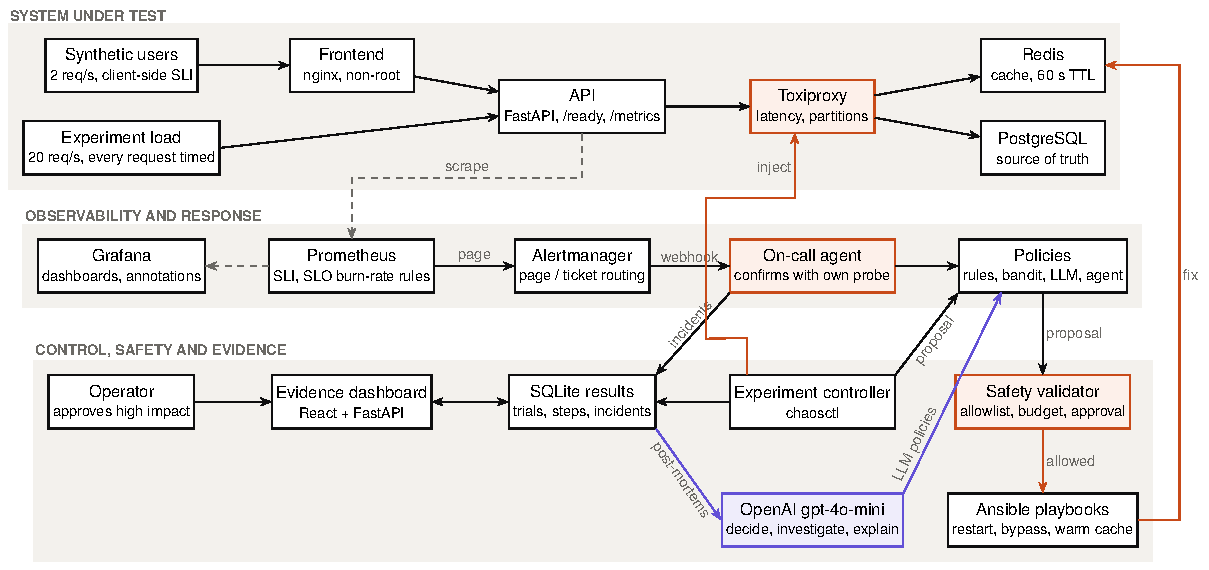
\includegraphics[width=\textwidth]{architecture.pdf}
\caption{\sys{} architecture. Faults enter through Toxiproxy (network) and Docker (process kills);
fixes enter through Ansible playbooks after the safety validator. The on-call agent is woken only by
Alertmanager; experiments are driven by the controller. All decisions and outcomes are stored in
SQLite and shown in the evidence dashboard; gpt-4o-mini is the only external service.}
\label{fig:arch}
\end{figure*}

Fig.~\ref{fig:arch} shows the three layers of \sys{}: the system under test, observability and
response, and control, safety and evidence. All components run as containers in one Docker Compose
project per lab; overlay files add host ports locally, an HTTPS proxy on servers, or a tunnel for
sharing. Each lab has a unique project name, so the CI pipeline can start isolated labs next to a
developer's lab on the same Docker host.

\subsection{System under test}
The target is a deliberately small shop: an nginx frontend, a FastAPI service and a catalogue of
1{,}000 items read with the cache-aside pattern from Redis (60\,s TTL) in front of PostgreSQL. Redis
calls time out after 500\,ms; database access uses a pool of 10 connections with 2\,s timeouts. A
Redis error yields HTTP~503 unless a \emph{cache-bypass} flag routes reads to PostgreSQL. The API
exposes liveness (\texttt{/health}), readiness with dependency probe latencies (\texttt{/ready}),
Prometheus metrics, and two administrative endpoints used by recovery actions. The API reaches both
data stores \emph{through Toxiproxy}~\cite{toxiproxy}, so latency and partitions can be injected
without touching the stores themselves.

\subsection{Faults}
Table~\ref{tab:faults} lists the seven faults. Five are used for training and design; two are
\emph{held out} and were run only after all policies were frozen. The partition is designed to look
like \act{redis\_down} to an observer while making a restart useless; the compound fault makes
cache bypass harmful.

\begin{table}[t]
\caption{Fault scenarios}
\label{tab:faults}
\centering
\small
\begin{tabular}{@{}lp{4.1cm}c@{}}
\toprule
Fault & Injection & Set \\
\midrule
\act{redis\_down} & kill the Redis container & train \\
\act{redis\_latency} & +800\,ms on Redis traffic ($>$ 500\,ms timeout) & train \\
\act{postgres\_latency} & +400\,ms on PostgreSQL traffic & train \\
\act{postgres\_down} & kill the PostgreSQL container & train \\
\act{api\_crash} & kill the API container & train \\
\midrule
\act{redis\_partition} & disable the Redis proxy (container healthy) & held out \\
\act{redis\_down\_slow\_db} & kill Redis and +400\,ms on PostgreSQL & held out \\
\bottomrule
\end{tabular}
\end{table}

\subsection{Load and recovery measurement}
\label{sec:measure}
Prometheus scrapes every 5\,s, too coarse for recoveries of 1--2\,s. During experiments an
\emph{open-model} load generator therefore sends 20 requests/s for random items regardless of
response times (a closed model would silently send less traffic during an outage) and records
the send time, completion time and status of every request (2\,s timeout).

Let requests be grouped into 1-second windows $w_i$ by send time after injection at $t_0$. A window
is \emph{healthy} if
\begin{equation}
\frac{|\{r \in w_i : r \text{ ok}\}|}{|w_i|} \ge 0.99 \;\wedge\; p_{95}(w_i) \le 300\,\text{ms},
\end{equation}
and empty windows are unhealthy. The service has \emph{recovered} once $k=5$ consecutive healthy
windows follow the first unhealthy window. To resolve recovery below window granularity, the
recovery time is the send time of the first request after the last \emph{bad} request (failed or
slower than 300\,ms) preceding that healthy run, minus $t_0$. A trial whose 10\,s pre-injection
baseline is unhealthy is marked invalid and excluded. These definitions are implemented in one
unit-tested module.

\subsection{Remediation loop and actions}
After detection (the last completed 1\,s window is unhealthy), the controller runs a loop modelled
on incident response: observe symptoms, ask the policy for an action, check it with the safety
validator, execute it, and wait up to 20\,s for three healthy seconds. If the service healed, the
step succeeded; otherwise the loop observes again, up to three executed actions per incident.
Policies see only \emph{symptoms}: error rate and p95 over the last second, whether the API answers,
and Redis/PostgreSQL reachability and probe latency from \texttt{/ready}; never the fault's name.

Actions are Ansible playbooks (Table~\ref{tab:actions}). Restarts locate containers by Compose
labels, refuse services outside an allowlist (\act{api}, \act{redis}, \act{postgres},
\act{frontend}), restart them and wait for readiness; \act{cache\_bypass} and \act{warm\_cache} call
the API's administrative endpoints (warming uses a dedicated database connection so that it does
not queue behind an exhausted pool).

\begin{table}[t]
\caption{Recovery actions, safety impact and reward cost}
\label{tab:actions}
\centering
\scriptsize
\setlength{\tabcolsep}{3.5pt}
\begin{tabular}{@{}lp{3.35cm}cc@{}}
\toprule
Action & Effect & Impact & Cost \\
\midrule
\act{restart\_redis} & restart Redis, await readiness & medium & 0.05 \\
\act{restart\_postgres} & restart PostgreSQL & high & 0.20 \\
\act{restart\_api} & restart the API & medium & 0.10 \\
\act{cache\_bypass} & serve reads from PostgreSQL & low & 0.05 \\
\act{warm\_cache} & load all items into Redis (10\,min) & low & 0.02 \\
\bottomrule
\end{tabular}
\end{table}

\subsection{Safety shield}
\label{sec:safety}
Every proposal, from every policy, is checked in order against a declarative policy file; the first
failing rule blocks it and the reason is recorded: (1)~the lab's project name must match an approved
pattern; (2)~the action must be on the allowlist; (3)~no action may repeat within an incident,
which prevents restart loops; (4)~at most three actions may execute per incident; (5)~high-impact
actions need approval. Approval is \emph{auto} (logged) in the isolated experiment lab, \emph{human}
in on-call mode, or \emph{deny}. The playbooks enforce their own service allowlist as an independent
second layer. A red-team policy proposes destructive and non-allowlisted actions on purpose.

\subsection{Policies}
\label{sec:policies}
\textbf{Runbook.} Restart whatever looks broken, then restart the API; a common operational default.

\textbf{Expert heuristic.} Rules written after studying the training results (e.g.\ PostgreSQL
probe $>$200\,ms $\Rightarrow$ \act{warm\_cache}; Redis unreachable $\Rightarrow$ \act{cache\_bypass}).

\textbf{LinUCB bandit.} The context $x \in \mathbb{R}^8$ contains a bias, binary indicators for API
down, Redis unreachable and PostgreSQL unreachable, log-scaled probe latencies
$\ell(m)=\min(\log(1+m)/\log(2001),1)$ for both stores, the error rate, and $\ell(p_{95})$. Each
executed step yields the reward
\begin{equation}
r = \max\!\left(0,\, 1 - \frac{t_{\text{heal}}}{20\,\text{s}}\right) - c(a),
\end{equation}
with $r=-c(a)$ if the step never healed and $c(a)$ the safety cost in Table~\ref{tab:actions}. For
each action $a$, disjoint LinUCB~\cite{li2010linucb} maintains $A_a = I + \sum x x^\top$ and
$b_a = \sum r\,x$, predicts $\hat\theta_a^\top x$ with $\hat\theta_a = A_a^{-1} b_a$, and scores
$\hat\theta_a^\top x + \alpha\sqrt{x^\top A_a^{-1} x}$ with $\alpha=0.5$. The model is trained
offline on logged steps of training faults only (an assertion rejects held-out data) and acts
greedily among actions not yet tried in the incident.

\textbf{LLM.} gpt-4o-mini~\cite{openai2024mini} receives the symptoms, the allowed actions with
descriptions, and what has already run or been blocked, and returns JSON with an action and a
one-sentence reason (temperature~0).

\textbf{LLM agent.} The same model and prompt, plus five tools: an instant PromQL query, the last
two minutes of a shop container's log (repeated lines collapsed), container states, the readiness
check, and \texttt{decide(hypothesis, action, reason)}. The agent must call at least one
investigation tool before \texttt{decide} is offered and is forced to decide after five. The fault
injector is invisible to all tools. Every call and result is stored as an auditable trail.

\textbf{Ablation variants.} Both LLM policies also exist with one added paragraph of generic SRE
guidance (restarts only fix crashed or hung processes, not slow or unreachable networks, and lose
warm state; check down vs.\ slow; prefer the least disruptive action; consider side effects). It
names no fault and no action.

\subsection{On-call mode}
\label{sec:oncall}
\begin{figure}[t]
\centering
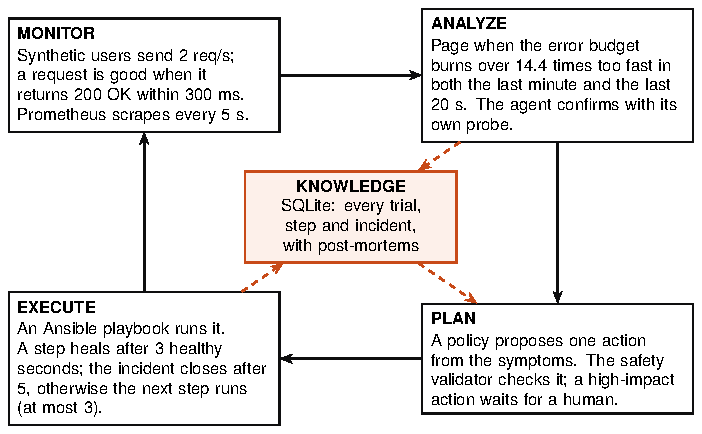
\includegraphics[width=\columnwidth]{loop.pdf}
\caption{The on-call loop mapped onto MAPE-K~\cite{kephart2003vision}.}
\label{fig:loop}
\end{figure}

Experiments know when and what they inject. On-call mode removes that knowledge (Fig.~\ref{fig:loop}).
A synthetic-user service sends 2 requests/s and counts each request as \emph{good} (200 within
300\,ms), \emph{slow} or \emph{error}; the SLI is measured at the client because the API cannot count
requests it never receives. The SLO is 99\% good requests, so the error budget is $\epsilon=0.01$.
With $\rho_w$ the bad-request ratio over window $w$, the burn rate is $\beta_w=\rho_w/\epsilon$.
Following the SRE Workbook~\cite{beyer2018workbook}, scaled from hours to lab time, Prometheus pages
when
\begin{equation}
\beta_{1\,\text{min}} > 14.4 \;\wedge\; \beta_{20\,\text{s}} > 14.4,
\end{equation}
raises a ticket when $\beta_{1\,\text{h}} > 3 \wedge \beta_{10\,\text{min}} > 3$, and raises a ticket
if the synthetic traffic itself is not scraped for 30\,s. These rules are unit-tested with
\texttt{promtool}: an outage pages and stops paging after recovery, a 5\,s blip does not page, and
slow responses burn budget like errors.

Alertmanager delivers pages to the agent's webhook (group wait 1\,s, repeat every minute) and
inhibits the slow-burn ticket while the page fires. On a page, the agent (i)~stands down if
autopilot is off or an experiment holds the shared lab lock; (ii)~sends its own probe traffic
(10 requests/s for 4\,s) and dismisses the page as stale if three consecutive seconds are healthy,
because windowed alerts lag behind reality; (iii)~opens an incident and runs the remediation loop
with a shield in \emph{human} approval mode: a high-impact proposal creates an approval request that
an operator approves or denies in the dashboard, only the first decision counts, and with no
decision in 60\,s the action is not run; (iv)~closes the incident only on sustained recovery (five
healthy windows), otherwise escalates to a human without retrying; an escalation closes
automatically once the service is healthy; and (v)~asks gpt-4o-mini for a post-mortem from the
incident record. The agent runs in its own container and never reads the chaos log, so every
incident is detected from symptoms alone. On the chaos side, the dashboard can inject a chosen or
random fault unannounced, a chaos monkey can inject random faults at jittered intervals, and every
injected fault is rolled back after five minutes. A scorecard matches each logged fault to the first
incident opened within ten minutes and reports time to alert, to engagement and to recovery.

\subsection{Evidence and generative AI}
All trials, steps (symptoms, verdict, timing, reward, the LLM's reason, the agent's trail), incidents,
approvals and faults are stored in SQLite on a shared volume. A React dashboard presents the fixed-action
matrix, policy rankings, the learning curve, per-incident timelines, the on-call console and the safety
log. gpt-4o-mini writes post-mortems and answers free-form questions strictly from the measured data;
it is never a source of numbers.

\subsection{CI/CD pipeline and DevSecOps}
\label{sec:cicd}
\begin{figure*}[t]
\centering
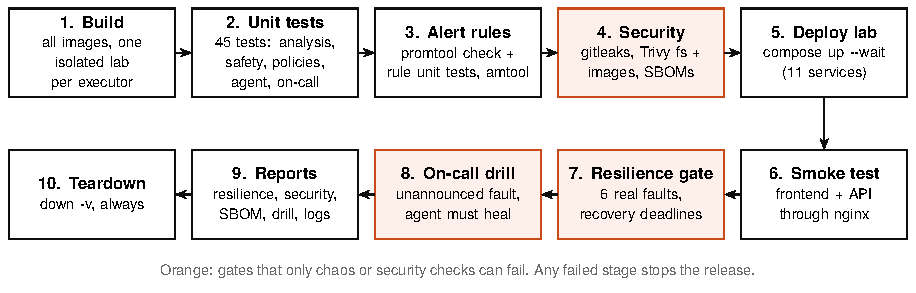
\includegraphics[width=0.86\textwidth]{pipeline.pdf}
\caption{The Jenkins pipeline. Every stage is a gate; the security scan, the resilience gate and the
on-call drill are the stages that only chaos or security findings can fail.}
\label{fig:pipeline}
\end{figure*}

A Jenkins multibranch job, defined as code, builds every branch (Fig.~\ref{fig:pipeline}). Each build
starts its own lab without host ports and tears it down afterwards. Besides unit tests and a smoke
test, four stages are specific to \sys{}: \emph{alert rules} (\texttt{promtool} and \texttt{amtool}
checks and rule unit tests); a \emph{security scan} with gitleaks over the working tree and the whole
git history, Trivy over pinned Python and npm dependencies (including build-time dependencies) and
Dockerfiles, and Trivy over every built image with a CycloneDX SBOM archived per image; a
\emph{resilience gate} that runs six real faults with a fixed action each and fails if recovery
exceeds a deadline (10--20\,s, about twice the locally measured median); and an \emph{on-call
drill} that kills Redis without notice and fails unless the agent heals it within 120\,s. Sources
reach scanners through standard input rather than bind mounts, because Jenkins drives the host's
Docker engine. A production overlay places Caddy in front of the dashboard as the only public entry
point (automatic HTTPS, bcrypt login, security headers), and an Ansible playbook provisions a fresh
Ubuntu server in one command; a Cloudflare tunnel shares a laptop lab behind the same login.

\section{Experimental Methodology}
\label{sec:method}
\textbf{Testbed.} All experiments ran on one laptop (Intel Core i5-12450H, 8 cores/12 threads, 16\,GB
RAM, Windows 11) with Docker Desktop 29.8 on WSL2 (12 vCPUs and 7.6\,GB for the Docker VM). The lab
comprises eleven long-running containers (frontend, API, Redis~7.2, PostgreSQL~16, Toxiproxy~2.9,
synthetic users, Prometheus~2.53, Alertmanager~0.27, Grafana~11.1, the on-call agent and the dashboard).
Recovery actions run with ansible-core~2.21; LLM policies use gpt-4o-mini at temperature~0.

\textbf{Trial protocol.} Each trial resets the lab (faults removed, stopped containers started,
readiness awaited, bypass off, Redis flushed), warms up for 15\,s at 20 requests/s, injects the fault,
detects the outage within 15\,s, runs the remediation loop, keeps the load running until recovery or
a timeout (60\,s for fixed actions, 90\,s for policies), and resets again. The synthetic users
(2 requests/s) and the on-call agent run throughout; the shared lab lock makes the agent stand down
during experiments.

\textbf{Studies.}
\begin{enumerate}
\item \emph{Fixed-action matrix}: every training fault $\times$ every action, two trials each. These
  trials also provide the bandit's first training data.
\item \emph{Policy comparison}: runbook, heuristic, bandit and LLM on the training faults (two
  trials each) and, after freezing the policies, on the held-out faults (three trials each).
\item \emph{Learning curve}: the bandit is replayed over all logged training steps in 30 random
  orders and, after every $k$ steps, scored on how often it selects the best measured action for each
  logged context; the runbook and heuristic are scored on the same contexts. The ``best'' action per
  fault is the one with the highest mean measured reward.
\item \emph{LLM ablation}: a $2\times2$ design over \{no tools, tools\} $\times$ \{no guidance, SRE
  guidance\}, two trials per fault and variant, all seven faults, run as one batch under identical
  conditions (\nAblation{} trials).
\item \emph{Safety}: red-team runs plus an audit of every blocked proposal across all studies.
\item \emph{On-call campaign}: each of the seven faults injected unannounced three times through the
  dashboard API, one at a time, with the heuristic responder. A scripted operator approves high-impact
  requests after a fixed 5\,s reaction time. After each fault the lab is reset and the next fault is
  injected only once no alert is firing.
\item \emph{CI/CD}: the pipeline on \texttt{main} and on a branch with a seeded one-character bug.
\end{enumerate}

\textbf{Metrics.} Recovery rate and recovery time (Section~\ref{sec:measure}); failed requests per
incident; best-action accuracy and regret for the learning curve; for on-call incidents, time to
alert (Prometheus alert start minus injection), time to engage (page received minus injection) and
time to recover (start of sustained healthy probe traffic minus injection).

\textbf{Reproducibility.} The repository contains the lab, the experiment CLI, the measurement
campaign script, and the scripts that regenerate every figure and table in this paper from the
experiment database.

\section{Results}
\label{sec:results}
Unless stated otherwise, cells report recovered/trials, the median recovery time in seconds and its
range; at 20 requests/s a 60\,s outage is about 1{,}200 failed requests. The database holds
\nTrials{} experiment trials.

\subsection{No single fix works everywhere}
\begin{figure}[t]
\centering
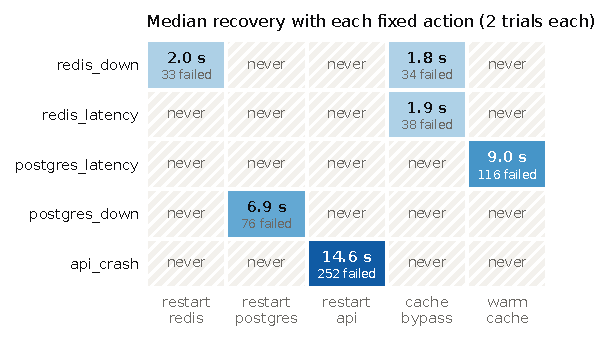
\includegraphics[width=\columnwidth]{fig_matrix.pdf}
\caption{Fixed-action matrix (two trials each): median recovery and mean failed requests per incident.
Hatched cells never recovered within the timeout.}
\label{fig:matrix}
\end{figure}

Fig.~\ref{fig:matrix} shows that every training fault has exactly one quickly recovering action, and
that it differs per fault. Restarting Redis cannot fix \act{redis\_latency} because Redis itself is
healthy; only \act{cache\_bypass} removes the slow path. \act{cache\_bypass} makes
\act{postgres\_latency} worse by sending every read to the slow database, whereas one bulk
\act{warm\_cache} query takes the database off the request path. Choosing a wrong action is not a
small penalty: the outage continues until the 60\,s timeout, costing 447--1{,}128 failed requests per
incident instead of 33--252.

\subsection{Policies on training and held-out faults}
\begin{table*}[t]
\caption{Policy comparison: recovered/trials, median recovery in seconds (range). Bold: fastest full
recovery per fault. Below the rule: held-out faults, run after the policies were frozen.}
\label{tab:policies}
\centering
\small
\begin{tabular}{@{}lcccc@{}}
\toprule
Failure & Runbook & Heuristic & Bandit & LLM \\
\midrule
\texttt{redis\_down} & 2/2, 2.9\,{\scriptsize(1.9--4.0)} & \textbf{2/2, 1.6} & 2/2, 1.6 & 2/2, 4.0 \\
\texttt{redis\_latency} & $\times$ 0/2 & 3/3, 2.8\,{\scriptsize(2.8--2.9)} & \textbf{2/2, 2.7\,{\scriptsize(2.7--2.8)}} & 2/2, 28.9\,{\scriptsize(5.0--52.9)} \\
\texttt{postgres\_latency} & $\times$ 0/2 & \textbf{2/2, 9.8\,{\scriptsize(9.7--9.8)}} & 2/2, 32.7\,{\scriptsize(10.1--55.2)} & $\times$ 0/2 \\
\texttt{postgres\_down} & \textbf{2/2, 7.4\,{\scriptsize(7.3--7.4)}} & 3/3, 8.0\,{\scriptsize(6.5--10.4)} & 2/2, 43.2\,{\scriptsize(8.0--78.5)} & 2/2, 12.0 \\
\texttt{api\_crash} & 2/2, 16.1\,{\scriptsize(16.0--16.2)} & \textbf{2/2, 16.0\,{\scriptsize(15.9--16.0)}} & 2/2, 16.0 & 2/2, 16.1\,{\scriptsize(16.1--16.2)} \\
\midrule
\texttt{redis\_partition} & $\times$ 0/3 & 3/3, 0.9\,{\scriptsize(0.8--1.1)} & \textbf{3/3, 0.8} & 3/3, 43.4\,{\scriptsize(43.4--43.5)} \\
\texttt{redis\_down\_slow\_db} & $\times$ 0/3 & $\times$ 0/3 & $\times$ 0/3 & $\times$ 0/3 \\
\midrule
\textit{recovered} & 6/16 & 15/18 & 13/16 & 11/16 \\
\bottomrule
\end{tabular}
\end{table*}

\begin{figure}[t]
\centering
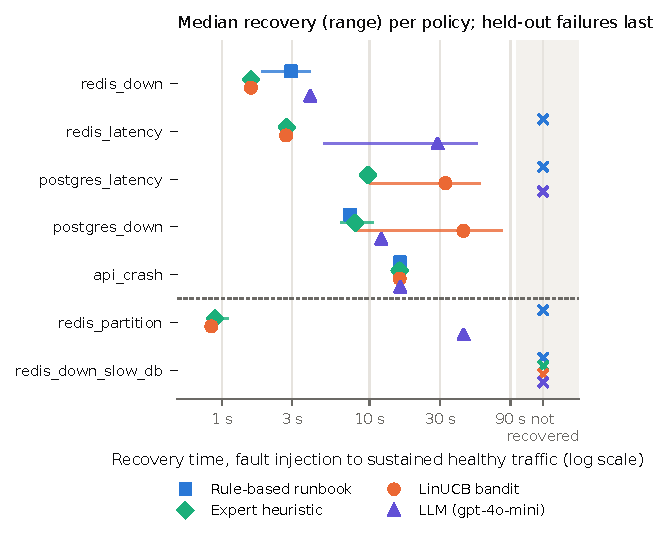
\includegraphics[width=\columnwidth]{fig_policies.pdf}
\caption{Median recovery (range) per policy on a log scale; $\times$ marks failures to recover.
Held-out faults are below the dashed line.}
\label{fig:policies}
\end{figure}

Table~\ref{tab:policies} and Fig.~\ref{fig:policies} compare the four main policies. The runbook
recovers only where restarting the broken-looking component is the right answer and fails on both
latency faults and on the partition. The expert heuristic, written after studying the training
results, recovers every training fault. The bandit, with no hand-written rules, matches the
heuristic's recovery rate; its two slow outliers (\act{postgres\_latency}, \act{postgres\_down}) come
from a first step chosen while connection-pool timeouts made a slow database look dead, after which
a second action healed the service. On the held-out partition, which looks exactly like a dead Redis
but cannot be fixed by a restart, the bandit generalises (3/3, 0.8\,s) while the runbook fails 0/3;
the LLM recovers but only after a restart attempt (43\,s). No policy recovers from the compound
fault, which requires two coordinated steps (restart Redis, then warm the cache, without bypass).

\subsection{The bandit learns from experience}
\begin{figure}[t]
\centering
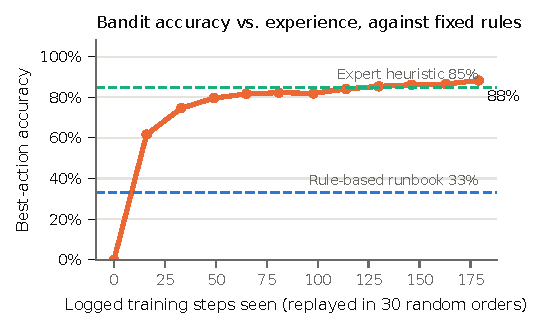
\includegraphics[width=\columnwidth]{fig_learning.pdf}
\caption{Best-action accuracy of the bandit as a function of logged steps seen (mean over 30 random
replay orders), against the fixed rules evaluated on the same contexts.}
\label{fig:learning}
\end{figure}

Replayed over all \lcSteps{} logged training steps, the bandit's best-action accuracy rises from 0
to \lcBandit{} (Fig.~\ref{fig:learning}), compared with \lcRunbook{} for the runbook and
\lcHeuristic{} for the expert heuristic on the same contexts. The pool contains every logged step
from the fixed-action matrix, the policy comparison and the LLM ablation, including unsuccessful
ones; an earlier snapshot with only the 52 fixed-action steps reached 98\%, against 40\% for the
runbook. The bandit thus reaches expert-level choices from logged outcomes alone.

\subsection{LLM ablation: tools versus advice}
\begin{table*}[t]
\caption{LLM ablation ($2\times2$, two trials per cell, one batch): recovered/trials, median recovery in
seconds (range). Bold: fastest full recovery per fault among the four variants.}
\label{tab:ablation}
\centering
\small
\begin{tabular}{@{}lcccc@{}}
\toprule
 & \multicolumn{2}{c}{No tools} & \multicolumn{2}{c}{Tools (agent)} \\
\cmidrule(lr){2-3}\cmidrule(lr){4-5}
Failure & no guid. & guidance & no guid. & guidance \\
\midrule
\texttt{redis\_down} & 2/2, 4.1\,{\scriptsize(4.0--4.2)} & \textbf{2/2, 3.1\,{\scriptsize(3.0--3.2)}} & 2/2, 15.6\,{\scriptsize(11.4--19.8)} & 2/2, 8.1\,{\scriptsize(6.9--9.2)} \\
\texttt{redis\_latency} & 2/2, 50.1\,{\scriptsize(50.0--50.2)} & \textbf{2/2, 3.3\,{\scriptsize(3.1--3.5)}} & 2/2, 58.6\,{\scriptsize(58.5--58.7)} & 2/2, 8.0\,{\scriptsize(7.7--8.3)} \\
\texttt{postgres\_latency} & $\times$ 0/2 & $\times$ 0/2 & $\times$ 0/2 & $\times$ 0/2 \\
\texttt{postgres\_down} & \textbf{2/2, 7.6\,{\scriptsize(7.2--8.0)}} & $\times$ 0/2 & 2/2, 17.1\,{\scriptsize(12.5--21.6)} & 2/2, 18.9\,{\scriptsize(15.4--22.4)} \\
\texttt{api\_crash} & \textbf{2/2, 13.2\,{\scriptsize(12.8--13.5)}} & 2/2, 44.1\,{\scriptsize(42.6--45.5)} & 2/2, 23.5\,{\scriptsize(23.2--23.7)} & 2/2, 22.1\,{\scriptsize(21.0--23.3)} \\
\midrule
\texttt{redis\_partition} & 2/2, 43.0\,{\scriptsize(42.5--43.5)} & \textbf{2/2, 2.3} & 2/2, 51.1\,{\scriptsize(50.9--51.3)} & 2/2, 28.0\,{\scriptsize(6.5--49.5)} \\
\texttt{redis\_down\_slow\_db} & $\times$ 0/2 & $\times$ 0/2 & $\times$ 0/2 & $\times$ 0/2 \\
\midrule
\textit{recovered} & 10/14 & 8/14 & 10/14 & 10/14 \\
\bottomrule
\end{tabular}
\end{table*}

\begin{figure}[t]
\centering
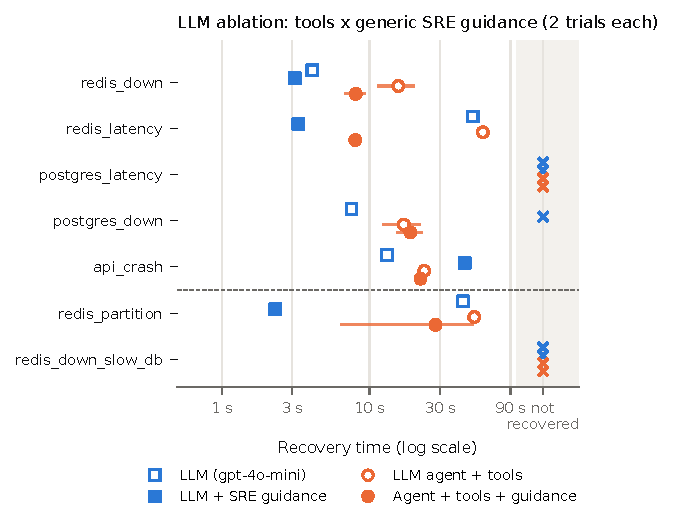
\includegraphics[width=\columnwidth]{fig_ablation.pdf}
\caption{LLM ablation. Squares: no tools; circles: tool-using agent. Hollow: no guidance; filled:
generic SRE guidance. Median recovery (range); $\times$: not recovered.}
\label{fig:ablation}
\end{figure}

Table~\ref{tab:ablation} and Fig.~\ref{fig:ablation} separate the two factors.
\emph{Advice changes the prior.} Without guidance, both LLM variants restarted first on every Redis fault,
which cost 43--59\,s on the two faults a restart cannot fix (\act{redis\_latency}, \act{redis\_partition}).
With the SRE paragraph and no tools, the model chose \act{cache\_bypass} first in \emph{all} 14 of its
trials. This was the fastest LLM behaviour in the study where bypass is right (\act{redis\_latency}
50.1\,s $\rightarrow$ 3.3\,s, \act{redis\_partition} 43.0\,s $\rightarrow$ 2.3\,s, medians) and harmful
where a restart is right: it never restarted the crashed database (0/2, against 2/2 in 7.6\,s without
advice) and bypassed the cache before restarting the crashed API (44.1\,s against 13.2\,s).

\emph{Tools alone cost time without changing decisions.} The tool-using agent called 3.6 tools per
decision on average (1--5, 45 decisions). Without guidance its first action matched the plain LLM's on
every fault except \act{postgres\_latency}, where neither helped, so the investigation added 8--12\,s per
incident (e.g.\ \act{redis\_down} 4.1\,s $\rightarrow$ 15.6\,s) without improving any outcome.

\emph{Together, they are the most robust configuration.} With tools and guidance the agent recovered
every fault that any LLM variant recovered (10/14). It bypassed the cache on Redis faults (8.0--8.1\,s)
and, unlike the guided model without tools, restarted the crashed database and API (18.9\,s and 22.1\,s):
on \act{postgres\_down} it queried readiness, dependency metrics and logs, stated the hypothesis
``PostgreSQL is down'', and restarted it. The guided model without tools saw the same reachability
symptom but bypassed the cache, so we attribute the difference to the investigation step (the extra
evidence, the explicit hypothesis, or both); two trials per cell cannot separate the two. One of its
two partition trials still restarted first (6.5\,s and 49.5\,s), a reminder that LLM behaviour varies at
temperature~0.

\emph{What no LLM found.} No variant used \act{warm\_cache} for \act{postgres\_latency} (0/8) or found the
two-step fix for the compound fault (0/8). The bandit and the expert heuristic, which learned from
measured outcomes, fix \act{postgres\_latency} reliably (Table~\ref{tab:policies}).



\subsection{Safety}
Across all studies, zero unsafe actions executed. In red-team runs the adversarial policy proposed
\act{drop\_database} (blocked: not an approved action), \act{restart\_grafana} (blocked: not
allowlisted) and repeated restarts (blocked: no repeats within an incident); only allowlisted
actions ran. The shield also constrained LLM behaviour: in the ablation, the tool-using agent twice
re-proposed \act{restart\_postgres} after it had already run on \act{postgres\_latency}, and both
proposals were blocked as repeats. In on-call mode, high-impact actions ran only after a recorded
human approval.

\subsection{On-call mode}
\begin{figure*}[t]
\centering
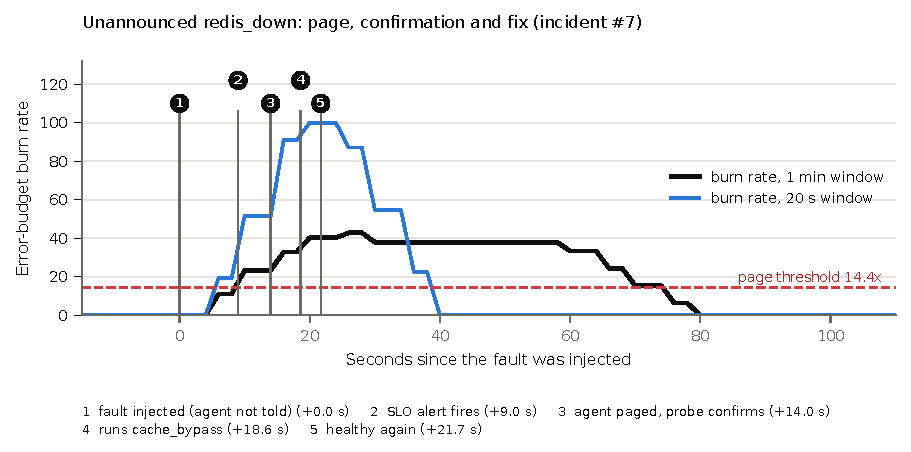
\includegraphics[width=0.92\textwidth]{fig_oncall_timeline.pdf}
\caption{An unannounced \act{redis\_down}, end to end. The 20\,s burn rate reacts first; the page
fires when the slower 1\,min window also exceeds 14.4 (multi-window rule). The agent confirms with
its own probe, runs \act{cache\_bypass}, and traffic is healthy about 24\,s after the fault; the alert
then clears as the windows drain.}
\label{fig:timeline}
\end{figure*}

\begin{table}[t]
\caption{On-call campaign: unannounced faults, three each, heuristic responder; medians in seconds
from injection to the alert, to the agent engaging, and to sustained healthy traffic.}
\label{tab:campaign}
\centering
\scriptsize
\setlength{\tabcolsep}{3pt}
\begin{tabular}{@{}lccccp{2.55cm}@{}}
\toprule
Failure & Healed & Alert & Engage & Healthy & Actions \\
\midrule
\texttt{redis\_down} & 3/3 & 10.2 & 14.7 & 21.7 & {\scriptsize cache\_bypass} \\
\texttt{redis\_latency} & 3/3 & 11.1 & 15.8 & 22.4 & {\scriptsize cache\_bypass} \\
\texttt{postgres\_latency} & 3/3 & 12.3 & 17.2 & 81.9 & {\scriptsize restart\_postgres,warm\_cache; warm\_cache} \\
\texttt{postgres\_down} & 3/3 & 14.5 & 19.0 & 34.7 & {\scriptsize restart\_postgres} \\
\texttt{api\_crash} & 3/3 & 12.8 & 17.4 & 36.3 & {\scriptsize restart\_api} \\
\midrule
\texttt{redis\_partition} & 3/3 & 11.5 & 16.1 & 21.0 & {\scriptsize cache\_bypass} \\
\texttt{redis\_down\_slow\_db} & 0/3 & 10.0 & 14.4 & -- & {\scriptsize cache\_bypass,restart\_postgres; cache\_bypass,restart\_postgres,restart\_redis} \\
\bottomrule
\end{tabular}
\end{table}

\begin{figure}[t]
\centering
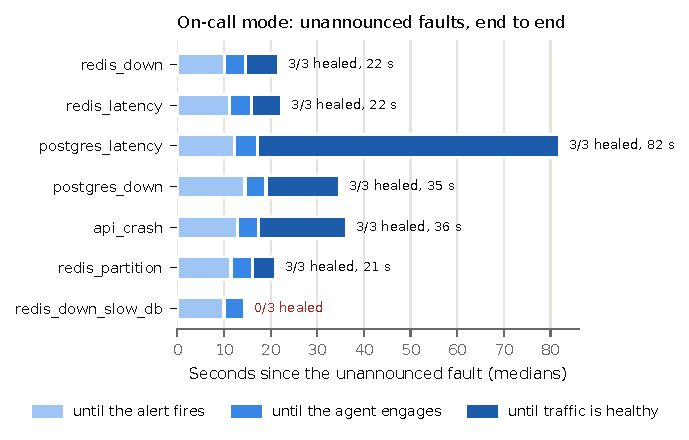
\includegraphics[width=\columnwidth]{fig_campaign.pdf}
\caption{On-call campaign, per fault: median time until the alert fires, the agent engages, and user
traffic is healthy again.}
\label{fig:campaign}
\end{figure}

Fig.~\ref{fig:timeline} traces one unannounced fault. Across the campaign
(Table~\ref{tab:campaign}, Fig.~\ref{fig:campaign}) the agent healed \ocHealed{} of \ocFaults{}
unannounced faults without being told what was injected. The median time from injection to the alert
was \ocMedDetect\,s, to the agent engaging \ocMedEngage\,s, and, for healed faults, to sustained healthy
traffic \ocMedRecover\,s; \ocEscalated{} incidents were escalated to a human, and \ocApprovals{}
high-impact actions ran only after the scripted operator's approval.
Detection was consistent across faults (10--15\,s to the alert, about 5\,s more until the agent was
paged and engaged), because it depends on the burn-rate windows rather than on the fault. Recovery
depended on the fix: about 21--22\,s for Redis faults healed by \act{cache\_bypass}, 35--36\,s for
crashed services that needed a restart (including the operator's 5\,s approval for
\act{restart\_postgres}). The slow database took longest (median 81.9\,s): pool timeouts made it look
unreachable, so the agent sometimes restarted PostgreSQL (with approval) before warming the cache,
the same ambiguity the bandit showed in experiments. All three compound faults were escalated after
the action budget was spent, and each escalation closed automatically once the lab was reset.

\begin{figure}[t]
\centering
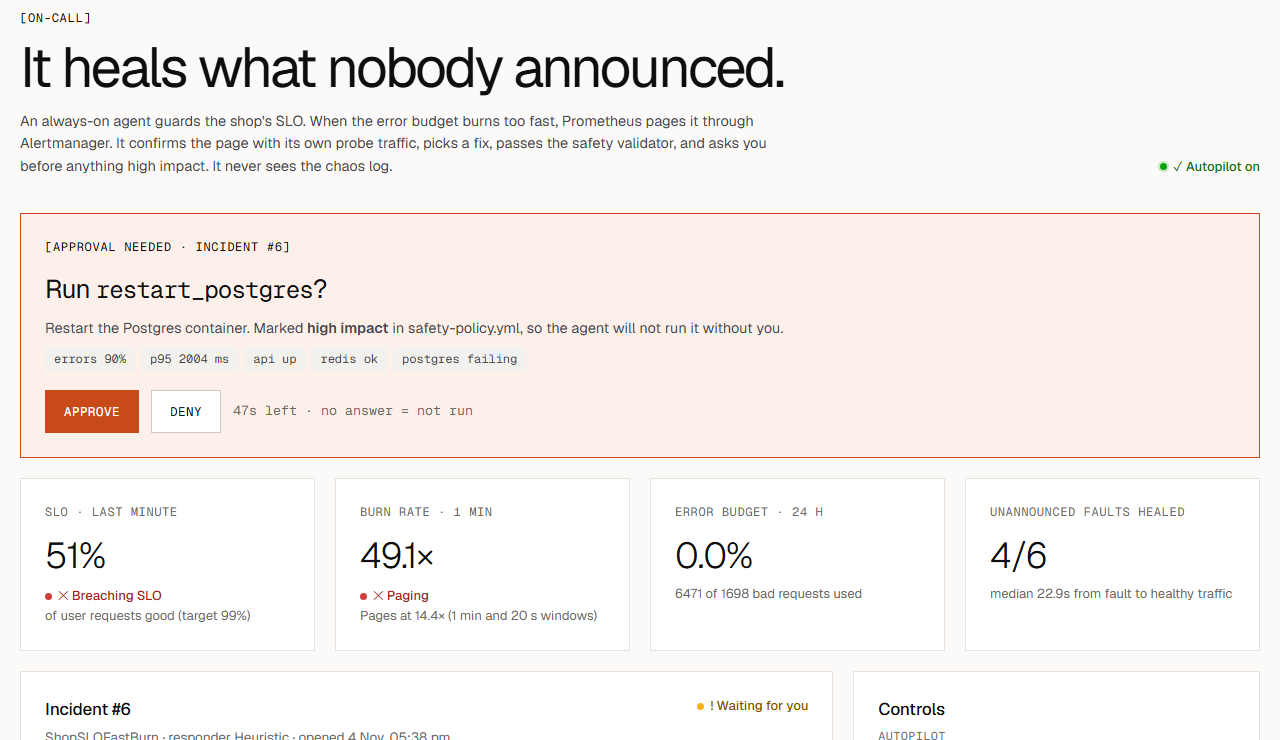
\includegraphics[width=\columnwidth]{screens/oncall-approval-crop.png}
\caption{The dashboard's on-call console during an unannounced \act{postgres\_down}: the agent proposes
the high-impact \act{restart\_postgres} and waits for a human decision; with no decision in 60\,s the
action is not run.}
\label{fig:approval}
\end{figure}



\subsection{CI/CD gates and DevSecOps}
\begin{table}[t]
\caption{First security scan and remediation}
\label{tab:security}
\centering
\scriptsize
\setlength{\tabcolsep}{3pt}
\begin{tabular}{@{}p{1.55cm}p{3.05cm}p{3.0cm}@{}}
\toprule
Check & Finding & Action \\
\midrule
Secrets (code + history) & none in any commit & custom rule for current OpenAI key formats \\
Python deps & ansible-core 2.17.5: 2 HIGH CVEs & upgraded to 2.21.6 \\
npm deps (incl.\ build) & Vite 5.4.10: 1 HIGH, 12 MED., 3 LOW; esbuild: 1 MED.; no lockfile & Vite 6.4.5; lockfile + \texttt{npm ci} \\
Dockerfiles & 12 images run as root (HIGH); 1 CRITICAL false positive & 7 made non-root; 5 justified, documented \\
Images & frontend base: 3 CRIT., 58 HIGH (old Alpine); Docker CLI, gosu: 1 CRIT.\ each (old Go) & nginx 1.30 + OS upgrade (0 left); CLI 29.8; gosu accepted, expires; SBOMs (441 comp.) \\
\bottomrule
\end{tabular}
\end{table}

A branch whose cache-bypass endpoint writes the wrong flag key (a one-character bug) returns HTTP~200
and reports success from its playbook. The security stage found no secrets but several fixable
issues (Table~\ref{tab:security}); after upgrades, non-root images, newer base images and documented
exceptions, the scan passes and now acts as a regression gate.
\begin{table}[t]
\caption{Jenkins stage durations for \texttt{main} and for the branch with the seeded bug ($\times$:
the failing stage; later stages do not run). The last stage includes teardown.}
\label{tab:ci}
\centering
\small
\begin{tabular}{@{}lrr@{}}
\toprule
Stage & \texttt{main} (s) & demo bug (s) \\
\midrule
Build images & 36 & 36 \\
Unit tests & 3 & 3 \\
Alert rules & 3 & 3 \\
Security scan & 43 & 42 \\
Deploy lab & 21 & 20 \\
Smoke test & 1 & 1 \\
Resilience gate & 178 & 290 $\times$ \\
On-call drill & 52 & -- \\
\midrule
Total & 346 & 409 \\
\bottomrule
\end{tabular}
\end{table}

Table~\ref{tab:ci} shows a full pipeline run. On \texttt{main} every stage passed in under six
minutes: the six gate checks recovered in 2.0--12.2\,s against deadlines of 10--20\,s, and in the
on-call drill the alert fired 8.9\,s after the unannounced fault, the agent engaged at 13.9\,s and
traffic was healthy at 19.6\,s. On the seeded-bug branch the same pipeline passed unit tests, alert
rules, the security scan and the smoke test, and failed the resilience gate on exactly the two
\act{cache\_bypass} checks (no recovery), while the other four checks passed.


\section{Discussion}
\label{sec:discussion}
\textbf{Measure before you automate.} The fixed-action matrix contradicts the default runbook: restarting
the component that looks broken is the right answer for only two of five training faults, and a
wrong action does not degrade gracefully, it prolongs the outage to the timeout. Any remediation
automation, human-written or learned, should be validated against measured outcomes.

\textbf{Learned policies generalise through symptoms.} Because the bandit sees symptoms rather than
fault names, it transfers to a fault it never saw when that fault presents like a known one but
needs a different fix than its look-alike's runbook (the partition). It does not compose actions:
the compound fault needs a two-step plan that a one-step learner cannot represent. The learner also
inherits ambiguity from its inputs: pool timeouts make a slow database look dead, which produced its
slow outliers.

\textbf{LLMs: priors, advice and evidence.} Without guidance, gpt-4o-mini behaves like the runbook: it
restarts first. One paragraph of generic SRE advice did not make the model reason case by case; it
replaced one prior with another (bypass first, in every trial). That helped exactly where restarts are
wrong and hurt where they are right, because a crashed service that times out looks like an unreachable
one in a symptom summary. An explicit investigation step (tools that query readiness, metrics and logs,
and a required hypothesis before deciding) let the advised agent tell the cases apart, making tools plus
advice the most robust LLM configuration, at a cost of seconds per decision. Tools without advice only
added time. No LLM configuration discovered that warming the cache fixes a slow database, a fix the
bandit and the expert both learned from measured outcomes. In this setting, LLMs contributed most as
explainers (post-mortems, questions answered from measured data) and as cautious first responders
behind a shield, and least as optimisers of recovery time; prompt content should be evaluated as
carefully as code, because a single generic paragraph moved recovery times by an order of magnitude in
both directions.

\textbf{Safety is layered.} The shield blocked every unsafe proposal, including repeats proposed by an
LLM agent, and the independent playbook allowlist would have stopped them again. In on-call mode the
human-approval path is fail-safe: silence means no action. The agent's ``confirm before acting'' and
``escalate instead of retrying'' rules prevented two classic automation failures: acting on stale
alerts and restart loops.


\textbf{Resilience as a release criterion.} The seeded bug shows why recovery deserves its own gate:
a remediation path can be syntactically correct, return success at every layer and still do nothing.
Only a test that injects the fault and measures user-visible recovery catches it. The same reasoning
applies to alerts: unit tests for burn-rate rules caught boundary behaviour (a 5\,s blip must not page)
that is otherwise discovered in production. The security stage found real, fixable problems on its
first run (vulnerable build-time dependencies, containers running as root), which illustrates that
DevSecOps gates pay off even in small projects.

\textbf{Threats to validity.} \emph{Internal:} all experiments ran on one laptop; absolute times
include Ansible and probing overhead and would differ on other hardware, but all policies share the
same conditions. Samples are small (two or three trials per cell), so we report ranges rather than
confidence intervals. LLM outputs vary between runs even at temperature~0. The synthetic users and
the on-call agent ran during the ablation but not during the earlier policy comparison, so we compare
LLM variants only within the ablation batch. \emph{Construct:} recovery thresholds (99\%, 300\,ms,
five windows) and the bandit's ``best action'' oracle (highest mean logged reward) are design choices;
other thresholds could change rankings near the boundaries. \emph{External:} the shop has one read
path, seven fault types and no write traffic; real systems have more failure modes, cascading effects
and noisier signals. The expert heuristic was written after seeing the training data, which favours
it on training faults.

\section{Conclusion and Future Work}
\sys{} shows that resilience can be treated like any other software property: specified (SLOs,
recovery deadlines, a safety policy), measured at request granularity, learned from, and enforced in
the release pipeline. Measuring every action against every fault overturned the default runbook; a
contextual bandit learned expert-level choices from logged outcomes and generalised to an unseen
fault through its symptoms; and a $2\times2$ ablation showed that, for gpt-4o-mini, generic advice
steers behaviour strongly in both directions, while tools contribute the evidence that makes the
advice safe to follow, at the price of decision time. An SLO-driven on-call agent closed the loop on
faults nobody announced, with a fail-safe human approval path, and a Jenkins pipeline made
resilience, alerting, security and on-call behaviour into release gates.

Future work follows from the limitations: sequence-aware policies (planning or reinforcement
learning behind the same shield) for compound faults; a Kubernetes port with Chaos Mesh and
SLO-gated canary releases; more trials with confidence intervals; safe online exploration in CI; and
distributed tracing as additional evidence for LLM agents. The lab, the measurement scripts and the
generators for every figure and table in this paper are open source.


\balance
\begin{thebibliography}{99}

\bibitem{basiri2016chaos}
A.~Basiri, N.~Behnam, R.~de~Rooij, L.~Hochstein, L.~Kosewski, J.~Reynolds, and C.~Rosenthal,
``Chaos engineering,'' \emph{IEEE Software}, vol.~33, no.~3, pp.~35--41, 2016.

\bibitem{principlesofchaos}
``Principles of chaos engineering,'' 2019. [Online]. Available: \url{https://principlesofchaos.org}

\bibitem{izrailevsky2011simian}
Y.~Izrailevsky and A.~Tseitlin, ``The Netflix Simian Army,'' Netflix Technology Blog, Jul. 2011.

\bibitem{beyer2016sre}
B.~Beyer, C.~Jones, J.~Petoff, and N.~R. Murphy, \emph{Site Reliability Engineering: How Google
Runs Production Systems}. Sebastopol, CA, USA: O'Reilly Media, 2016.

\bibitem{beyer2018workbook}
B.~Beyer, N.~R. Murphy, D.~K. Rensin, K.~Kawahara, and S.~Thorne, \emph{The Site Reliability
Workbook: Practical Ways to Implement SRE}. Sebastopol, CA, USA: O'Reilly Media, 2018.

\bibitem{forsgren2018accelerate}
N.~Forsgren, J.~Humble, and G.~Kim, \emph{Accelerate: The Science of Lean Software and DevOps}.
Portland, OR, USA: IT Revolution Press, 2018.

\bibitem{humble2010continuous}
J.~Humble and D.~Farley, \emph{Continuous Delivery: Reliable Software Releases through Build, Test,
and Deployment Automation}. Boston, MA, USA: Addison-Wesley, 2010.

\bibitem{kephart2003vision}
J.~O. Kephart and D.~M. Chess, ``The vision of autonomic computing,'' \emph{Computer}, vol.~36,
no.~1, pp.~41--50, 2003.

\bibitem{dang2019aiops}
Y.~Dang, Q.~Lin, and P.~Huang, ``AIOps: Real-world challenges and research innovations,'' in
\emph{Proc. IEEE/ACM 41st Int. Conf. Software Engineering: Companion}, 2019, pp.~4--5.

\bibitem{notaro2021survey}
P.~Notaro, J.~Cardoso, and M.~Gerndt, ``A survey of AIOps methods for failure management,''
\emph{ACM Trans. Intelligent Systems and Technology}, vol.~12, no.~6, 2021.

\bibitem{li2010linucb}
L.~Li, W.~Chu, J.~Langford, and R.~E. Schapire, ``A contextual-bandit approach to personalized news
article recommendation,'' in \emph{Proc. 19th Int. Conf. World Wide Web}, 2010, pp.~661--670.

\bibitem{ahmed2023recommending}
T.~Ahmed, S.~Ghosh, C.~Bansal, T.~Zimmermann, X.~Zhang, and S.~Rajmohan, ``Recommending root-cause
and mitigation steps for cloud incidents using large language models,'' in \emph{Proc. IEEE/ACM 45th
Int. Conf. Software Engineering}, 2023.

\bibitem{chen2024rcacopilot}
Y.~Chen \emph{et al.}, ``Automatic root cause analysis via large language models for cloud
incidents,'' in \emph{Proc. 19th European Conf. Computer Systems (EuroSys)}, 2024.

\bibitem{roy2024agents}
D.~Roy \emph{et al.}, ``Exploring LLM-based agents for root cause analysis,'' in \emph{Companion
Proc. 32nd ACM Int. Conf. Foundations of Software Engineering}, 2024.

\bibitem{yao2023react}
S.~Yao, J.~Zhao, D.~Yu, N.~Du, I.~Shafran, K.~Narasimhan, and Y.~Cao, ``ReAct: Synergizing reasoning
and acting in language models,'' in \emph{Proc. Int. Conf. Learning Representations}, 2023.

\bibitem{openai2024mini}
OpenAI, ``GPT-4o mini: Advancing cost-efficient intelligence,'' Jul. 2024. [Online]. Available:
\url{https://openai.com/index/gpt-4o-mini-advancing-cost-efficient-intelligence/}

\bibitem{alshiekh2018shielding}
M.~Alshiekh, R.~Bloem, R.~Ehlers, B.~K{\"o}nighofer, S.~Niekum, and U.~Topcu, ``Safe reinforcement
learning via shielding,'' in \emph{Proc. AAAI Conf. Artificial Intelligence}, 2018.

\bibitem{toxiproxy}
Shopify, ``Toxiproxy: A TCP proxy to simulate network and system conditions.'' [Online]. Available:
\url{https://github.com/Shopify/toxiproxy}

\bibitem{chaosmesh}
Chaos Mesh Authors, ``Chaos Mesh: A chaos engineering platform for Kubernetes.'' [Online].
Available: \url{https://chaos-mesh.org}

\bibitem{litmus}
LitmusChaos Authors, ``LitmusChaos: Open source chaos engineering platform.'' [Online]. Available:
\url{https://litmuschaos.io}

\bibitem{ntia2021sbom}
National Telecommunications and Information Administration, ``The minimum elements for a software
bill of materials (SBOM),'' U.S. Dept. of Commerce, Jul. 2021.

\end{thebibliography}


\end{document}
